\documentclass[portrait,final,archA0,fontscale=0.3]{baposter}

\usepackage{etoolbox}
\patchcmd{\thebibliography}{\section*{\refname}}{}{}{}
\usepackage{calc}
\usepackage{graphicx}
\usepackage{amsmath}
\usepackage{amssymb}
\usepackage{relsize}
\usepackage{multirow}
\usepackage{rotating}
\usepackage{bm}
\usepackage{url}
\usepackage{color}

\usepackage{graphicx}
\usepackage{multicol}

%\usepackage{times}
%\usepackage{helvet}
%\usepackage{bookman}
\usepackage{palatino}

\newcommand{\captionfont}{\footnotesize}

\setlength{\columnsep}{1.5em}
\setlength{\columnseprule}{0mm}


\newcommand{\compresslist}{%
\setlength{\itemsep}{1pt}%
\setlength{\parskip}{0pt}%
\setlength{\parsep}{0pt}%
}



\begin{document}



\definecolor{stevensred}{rgb}{0.6392,0.149,0.2196}
\definecolor{stevensgray}{rgb}{0.60392, 0.596, 0.60392}
\definecolor{airforceblue}{rgb}{0.36, 0.54, 0.66}

%%
\begin{poster}%
  % Poster Options
  {
  % Show grid to help with alignment
  grid=false,
  % Column spacing
  colspacing=1em,
  % Color style
  bgColorOne=white,
  borderColor=green,
  headerColorOne=orange,
  headerColorOne=orange,
  headerFontColor=black,
  boxColorOne=white,
  % Format of textbox
  textborder=rectangle,
  % Format of text header
  eyecatcher=true,
  headerborder=closed,
  headerheight=0.1\textheight,
%  textfont=\sc, An example of changing the text font
  headershape=rectangle,
  headershade=shadelr,
  headerfont=\Large\bf\textsc, %Sans Serif
  textfont={\setlength{\parindent}{1.5em}},
  boxshade=plain,
%  background=shade-tb,
  background=plain,
  linewidth=2pt
  }
  % Eye Catcher
  {\begin{minipage}{8em}
   \hfill\vspace{1in}
  \end{minipage} } % Empty space, replace with image if desired
  % Title
  {\bf \textsc{  Measurement Device Independence \\ A spy's worst enemy  } }
  % Authors
  {\textsc{  Chris Irish and Jonathan Gough \\ Department of Physics and Astronomy}}
  % University logo
  {% The makebox allows the title to flow into the logo, this is a hack because of the L shaped logo.
    
\includegraphics[height=9.0em]{img/ucl_logo}
  }

%%%%%%%%%%%%%%%%%%%%%%%%%%%%%%%%%%%%%%%%%%%%%%%%%%%%%%%%%%%%%%%%%%%%%%%%%%%%%%
%%% Now define the boxes that make up the poster
%%%---------------------------------------------------------------------------
%%% Each box has a name and can be placed absolutely or relatively.
%%% The only inconvenience is that you can only specify a relative position 
%%% towards an already declared box. So if you have a box attached to the 
%%% bottom, one to the top and a third one which should be in between, you 
%%% have to specify the top and bottom boxes before you specify the middle 
%%% box.
%%%%%%%%%%%%%%%%%%%%%%%%%%%%%%%%%%%%%%%%%%%%%%%%%%%%%%%%%%%%%%%%%%%%%%%%%%%%%%
    %
    % A coloured circle useful as a bullet with an adjustably strong filling
    \newcommand{\colouredcircle}{%
      \tikz{\useasboundingbox (-0.2em,-0.32em) rectangle(0.2em,0.32em); \draw[draw=black,fill=lightblue,line width=0.03em] (0,0) circle(0.18em);}}

%%%%%%%%%%%%%%%%%%%%%%%%%%%%%%%%%%%%%%%%%%%%%%%%%%%%%%%%%%%%%%%%%%%%%%%%%%%%%%
  \headerbox{Introduction}{name=Introduction,column=0,row=0}{
%%%%%%%%%%%%%%%%%%%%%%%%%%%%%%%%%%%%%%%%%%%%%%%%%%%%%%%%%%%%%%%%%%%%%%%%%%%%%%
Introduction Introduction Introduction Introduction Introduction Introduction Introduction Introduction Introduction Introduction Introduction Introduction Introduction Introduction Introduction Introduction Introduction Introduction Introduction Introduction Introduction Introduction Introduction Introduction Introduction Introduction Introduction Introduction Introduction Introduction Introduction Introduction Introduction Introduction Introduction Introduction Introduction Introduction Introduction Introduction Introduction Introduction Introduction Introduction Introduction Introduction Introduction Introduction Introduction Introduction Introduction Introduction Introduction Introduction Introduction Introduction Introduction Introduction Introduction Introduction

}

%%%%%%%%%%%%%%%%%%%%%%%%%%%%%%%%%%%%%%%%%%%%%%%%%%%%%%%%%%%%%%%%%%%%%%%%%%%%%%
  \headerbox{References}{name=references,column=0,above=bottom}{
%%%%%%%%%%%%%%%%%%%%%%%%%%%%%%%%%%%%%%%%%%%%%%%%%%%%%%%%%%%%%%%%%%%%%%%%%%%%%%

\bibliographystyle{unsrt}  
\bibliography{references}

}

%%%%%%%%%%%%%%%%%%%%%%%%%%%%%%%%%%%%%%%%%%%%%%%%%%%%%%%%%%%%%%%%%%%%%%%%%%%%%%
  \headerbox{Quantum Key Distribution}{name=Quantum Key Distribution,column=0,below=Introduction, above=references}{
%%%%%%%%%%%%%%%%%%%%%%%%%%%%%%%%%%%%%%%%%%%%%%%%%%%%%%%%%%%%%%%%%%%%%%%%%%%%%%
Quantum Key Distribution Quantum Key Distribution Quantum Key Distribution Quantum Key Distribution Quantum Key Distribution Quantum Key Distribution 
Quantum Key Distribution Quantum Key Distribution Quantum Key Distribution Quantum Key Distribution Quantum Key Distribution Quantum Key Distribution 
Quantum Key Distribution Quantum Key Distribution Quantum Key Distribution Quantum Key Distribution Quantum Key Distribution Quantum Key Distribution 
Quantum Key Distribution Quantum Key Distribution Quantum Key Distribution Quantum Key Distribution Quantum Key Distribution Quantum Key Distribution 
Quantum Key Distribution Quantum Key Distribution Quantum Key Distribution Quantum Key Distribution Quantum Key Distribution Quantum Key Distribution 
Quantum Key Distribution Quantum Key Distribution Quantum Key Distribution Quantum Key Distribution Quantum Key Distribution Quantum Key Distribution 
Quantum Key Distribution Quantum Key Distribution Quantum Key Distribution Quantum Key Distribution Quantum Key Distribution Quantum Key Distribution 
Quantum Key Distribution Quantum Key Distribution Quantum Key Distribution Quantum Key Distribution Quantum Key Distribution Quantum Key Distribution 

}

%%%%%%%%%%%%%%%%%%%%%%%%%%%%%%%%%%%%%%%%%%%%%%%%%%%%%%%%%%%%%%%%%%%%%%%%%%%%%%
\headerbox{Alice Has A Secret}{name=Alice Has A Secret,column=1,span=2,row=0}{
%%%%%%%%%%%%%%%%%%%%%%%%%%%%%%%%%%%%%%%%%%%%%%%%%%%%%%%%%%%%%%%%%%%%%%%%%%%%%%

\begin{center}
    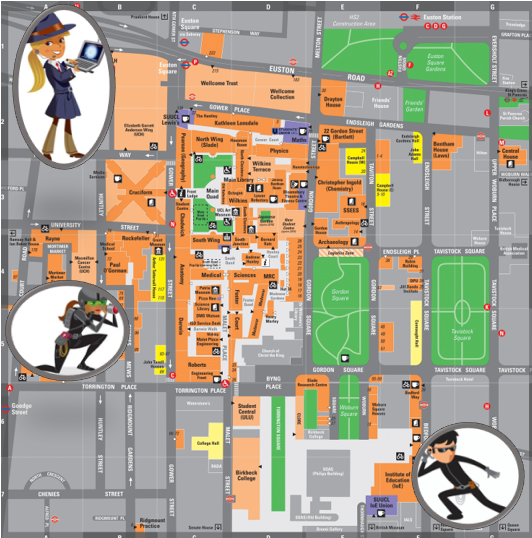
\includegraphics[width=\linewidth]{img/combined} 
\end{center}  

}

%%%%%%%%%%%%%%%%%%%%%%%%%%%%%%%%%%%%%%%%%%%%%%%%%%%%%%%%%%%%%%%%%%%%%%%%%%%%%%
  \headerbox{Measurement Device Independence}{name=Measurement Device Independence,column=1, span=2,below=Alice Has A Secret, above=bottom}{
%%%%%%%%%%%%%%%%%%%%%%%%%%%%%%%%%%%%%%%%%%%%%%%%%%%%%%%%%%%%%%%%%%%%%%%%%%%%%%


\noindent Alice and Bob are sick of having their secrets found out by Eve. Bob suggests they try a new approach, \textit{Measurement Device Independent Quantum Key Distribution}. Instead of sending there secrets directly to each other, they send them to a third party (Charlie). Charlie can combine Alice and Bobs information and perform a operation unique to quantum physics, called a Bell Measurement. The bell state measurement provides a vital piece of information that when combined with Alice and Bobs information, it allows them to work out what information is being sent to them. As only Alice/Bob knows her/his outgoing information, only they can know what information is being passed through the network.

\vspace{0.3cm}

\noindent However Bob has had one to many cranberry juices/Barnsley Bitters and can no longer remember what he sent to Alice. Just like Eve, Bob is now locked out of the network as Charlie can no longer verify him as a network user. Silly forgetful Bob!  

\begin{center}
    
\includegraphics[width=0.45\linewidth]{img/drunk_spy} 
\end{center} 

}


\end{poster}

\end{document}

